\documentclass[../main.tex]{subfiles}
\graphicspath{{\subfix{../IMAGES/}}}


\begin{document}
\localtableofcontents

\subsection{General measurement principles}
The physical variable is the \textbf{measurand}. A typical measurement system has three main components : \begin{enumerate}
    \item Sensing element : has a physical characteristic that responds to changes in the measurand (i.e. thermocouple that outputs millivolt depending on temperature)\\
    \item Signal conditioning element : converts the signal from the sensing element to a more suitable form for presentation or recording (i.e. amplifier, analog-to-digital)\\
    \item Signal presentation element : presents the measured value in a form which can be easily recognised by the observer (i.e. alphanumeric display)\\
\end{enumerate}

\begin{itemize}
    \item Range : input range of a sensing element is specified by the minimum and maximum values of its input. output range is specified by the minimum and maximum values of its output\\
    \item Span : maximum variation in input or output\\
    \item Resolution : smallest value that can be measured\\
    \item Dynamic range : ratio of its measurement span to its resolution\\
\end{itemize}

\quad \underline{Measurement accuracy or uncertainty :}\\

A measurement error : 
\begin{itemize}
    \item does not imply we made a mistake\\
    \item indicates that our measurement system is imperfect\\
\end{itemize}

The \textbf{uncertainty/accuracy} is a numerical estimate of the possible range of the error in a measurement. The error is not known exactly since the true value is not known. We should know the error bounds or uncertainty (the plus or minus range around the measured value).\\

\textbf{Accuracy} is either expressed as a percentage of full span (FS) or percentage of the reading + some integer-multiple of the least significant digit.\\

\textbf{Sensitivity} is defined as the change in output signal per unit change of input signal. High sensitivity means that small variations in the input signal give large changes in the output signal.\\

There exists multiple categories of errors : \\
\begin{itemize}
    \item Gross errors : made by human by mistake (avoidable, i.e. typos)\\
    \item System errors : \begin{itemize}
        \item Systematic/bias errors : (repeatable) $B = \varepsilon_s = \overline{Y}-X$\\
        \item Random/precision errors : (can not be predicted) $P = \varepsilon_r = Y-\overline{Y}$\\
    \end{itemize}
\end{itemize}

\quad \underline{Systematic errors :}\\
\begin{itemize}
    \item Loading errors : disturbances from the measurement process itself. Sensing element interferes with the measurand\\
    \item Calibration errors : incorrect estimates of the calibration curve\\
    \item Hysterisis errors : differences between an upscale sequential test and a downscale sequential test\\
    \item Fixed offsets : constant values that are added to all the measurements, independent of the measurement\\
\end{itemize}

\quad \underline{Random errors :}\\
Scatter in measurement data is an indicator of random error and can be caused by a number of factors (temperature, humidity, vibrations...). The random error bands can be estimated by statistical analysis of the repeated measurements.\\

\quad \underline{Precision vs Accuracy :}\\

Precision is the spread around the measured value, accuracy is the distance from the measured value to the true value.\\

A measurement system that has a low random error is considered precise. Yet, a precise system is not necessarily accurate.\\

\begin{itemize}
    \item High repeatability gives low random error but no direct indication of accuracy\\
    \item High accuracy means low random and systematic errors\\
    \item Systematic and random errors lead to poor accuracy.\\
\end{itemize}


\subsection{Fluid velocity measurements}
An anemometer is an instrument for measuring the speed and direction of a flow. Anemometry is the technique of measuring wind speed and direction. Velocimetery is the techniques of measuring the velocity of fluids.
All measurements (except PIV) are intrusive and need to be placed within the flow.

\subsubsection{Rotating mechanical flow meters}
A cup anemometer tends to equal forces acting on the cups : $F_{top} = F_{bottom}$ : $C_{D,top} \frac{1}{2} \rho A (U_{wind} + \omega R)^2 = C_{D,bottom} \frac{1}{2} \rho A (U_{wind} - \omega R)^2 \Rightarrow U_{wind} = \omega R \frac{\sqrt{C_{D,top}} + \sqrt{C_{D,bot}}}{\sqrt{C_{D,bot}} - \sqrt{C_{D,top}}}$.
With $C_D$ the drag coefficient.\\

\subsubsection{Pressure-based velocity measurements}
From Bernoulli equation : $\frac{dp}{p} + UdU = 0$ along a streamline. We have $p_0-p = \frac{1}{2} \rho U_{wind}^2$ in Pitot tube.\\

With Prandtl tube, we also retrieve the static pressure : $U_{\infty} = \sqrt{\frac{2(p_0-p_{static})}{\rho}}$\\

\subsubsection{Thermal anemometry}
Heat is introduced in the sensor by Joule heating and lost by forced convection.\begin{itemize}
    \item In steady flow : $R_w I_w^2 = (T_w-T_f) \phi_{conv}(U)$\\
    \item In unsteady flow : $m_w c_w \frac{T_w}{dt} = R_w I_w^2 - (T_w-T_f) \phi_{conv}(U)$\\
\end{itemize}
With constant current, a change in U creates a change in $R_w$. With constant temperature, a change in U creates a change in $I_w$. With constant voltage, a change in U creates a change in $I_w$.\\


\subsubsection{Particle-based velocimetry}
These techniques are indirect, determine the particle velocity instead of the fluid velocity. A source of error is the mismatch between the densities of the fluid and the tracer particle.\\
Effect of gravity on the tracer particle : $\Vec{U}_g = d_p^2 \frac{\rho_p-\rho}{18\mu} \Vec{g}$.\\
This generates a lag between the tracer particles and the fluid flow : $\Vec{U}_s = d_p^2 \frac{\rho_p - \rho}{18\mu} \Vec{a}$.\\

\quad \underline{Laser Doppler anemometry :}\\
Two laser beams are send on the fluid at a specific location. When a particle crosses the beams trajectory, it generates a peak in intensity that can be retrieved by the receiver.\\

\quad \underline{Particle Image Velocimetry :}\\
We have mono PIV when one camera makes a 2D plane of the fluid flow. Stereo PIV with two cameras at an angle to generates a 2D plane of the fluid flow with 3 components.\\
A cross-correlation is used to find the path of particle between two images. Need to define interrogation windows. The cross-correlation is defined as $C(\Delta x, \Delta y) = \int \int I_1(x,y) I_2(x+\Delta x, y+\Delta y) dxdy$.\\
The image magnification factor M correct for lens distortions and provide a factor between a length and a number of pixels.\\
$u = \frac{\Delta x}{M} \frac{1}{\Delta t}$, with $[\Delta x] = px$ and $[\Delta t] = s$.\\

The size of interrogation window depends on the flow, seeding, imaging and timing. Too small interrogation window size lead to not enough particles and too large interrogation window decrease spatial resolution.\\

\quad \underline{Advanced correlation techniques :}\\
Window shift technique. Multi-grid interrogation to find the best size of interrogation window.\\

Partial overlap in particle image lead to broad peak and a Gaussian bell fit. Full overlap or no overlap at all lead to single peak and a Gaussian bell fit.\\

\subsection{Strain gauge measurements}
Strain is the amount of deformation of a body : $\varepsilon = \frac{\Delta L}{L}$.\\
The Gauge factor (sensitivity) is defined as $GF = \frac{\Delta R/R}{\varepsilon} \simeq 2$ in general.\\
A strain gauge is sensitive to a change in length but also in a change in temperature.\\
The Wheatstone bridge consists on four resistance in a square shape with an exciting voltage and an output voltage $V_0$ given by : $V_0 = [\frac{R_3}{R_3+R_4} - \frac{R_2}{R_1+R_2}] V_{ex}$.\\
It is referred as a balanced bridge if $\frac{R_1}{R_2} = \frac{R_4}{R_3}$ as $V_0=0$.\\
The quarter bridge uses a potentiometer as one of the resistance. The governing equation is therefore : $\frac{V_0}{V_{ex}} = -\frac{GF \varepsilon}{4} (\frac{1}{1+GF \varepsilon/2})$.\\
The half bridge uses two potentiometer. The temperature effect is compensated and we have the governing equation : $\frac{V_0}{V_{ex}} = -\frac{GF \varepsilon}{2}$.\\
The full bridge uses four potentiometer. The effect of temperature is compensated and the governing equation is :$\frac{V_0}{V_{ex}} = -GF \varepsilon$.\\

\begin{itemize}
    \item Bending strain : $\varepsilon \propto M = FL$, $R_1, R_3$ on the face of the force and $R_2, R_4$ on the other face.\\
    \item Axial strain : $\varepsilon \propto \sigma = \frac{F}{bh}$, $R_1, R_3$ aligned with F and $R_2, R_4$ perpendicular to the force.\\
    \item Shear strain : $\gamma \propto \tau = \frac{FQ}{bI}$ $R_1,R_2$ in a cross pattern on the side face, same for $R_3, R_4$\\
    \item Torsional strain : $\gamma \propto \tau = \frac{Md/2}{J}$, same configuration as for shear strain.\\
\end{itemize}

We have a linear relation between forces and measured volts : $[F] = [R] [V_0]$.\\
To find $[R]$, solve $[V_{cali}] = [R]^{-1} [F_{cali}]$ for R using linear regression.

\subsection{Motion and Vibration}
\subsubsection{Strain gauges}
The electrical resistance is given by : $R = \rho \frac{L}{w t}$. For an unclamped metal pad in uni-axial loading : $\frac{\delta R}{R_0} = \varepsilon (1+2\nu)$.\\
To measure resistance, we convert it to voltage. For this, we can use a Wheatstone Bridge comprising 4 strain gauge.

\begin{figure}[hbt!]
    \centering
    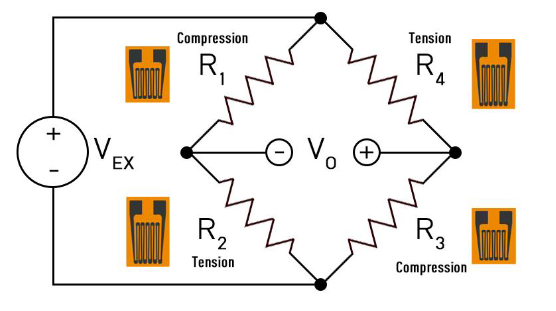
\includegraphics[width = .5\textwidth]{IMAGES/mecavib/Screenshot from 2024-06-08 12-12-52.png}
\end{figure}

For this setup, we have $\frac{\delta V}{V_{bias}} = \frac{\delta R}{R_0}$. In general, we only have one resistor as strain gauge to mitigate the effect of compensation between the strain gauges (difference in voltage is divided by four).\\

\begin{itemize}
    \item Advantages : accuracy and lifetime stability\\
    \item Disadvantages : fixing/gluing technique of gage to structure is critical, require compensation of temperature\\
\end{itemize}

\subsubsection{Motion (Eddy current)}
Changing magnetic field induces loops of electrical current within conductors.\\
A sending coil generates a primary magnetic field which generates eddy currents in the object approaching (if conductor) which in turns generates a magnetic field in the opposite direction and reduce the impedance of the receiving coil.\\

\begin{itemize}
    \item Advantages : high temperature stability, resistant to pressure/dirt/oil, can operate at high pressure, wear-free, non-contact sensors for measuring displacement and position in harsh environments\\
\end{itemize}

\subsubsection{Velocity (Laser Doppler Vibrometer)}
The frequency emitted by a moving object depends on its velocity according to :\begin{equation}
    f = (\frac{c\pm v_r}{c\pm v_s}) f_0
\end{equation}
With : \begin{itemize}
    \item $f$ : measured frequency\\
    \item $c$ : speed of propagation of waves\\
    \item $v_r$ : velocity of receiver\\
    \item $v_s$ : velocity of sender\\
    \item $f_0$ : emitted frequency\\
\end{itemize}

\begin{itemize}
    \item Advantages : high sensitivity, non-contact method, environment flexibility, no mass loading\\
    \item Limitations : single-axis measurements, complex setup, portability, need reflective surface\\
\end{itemize}

\subsubsection{Accelerometers}
We use inertial sensors. Three types of accelerometer : capacitive, piezoresistive and piezoelectric.\\

\quad \underline{Piezoresistive accelerometers :}\\
Measure the resistance changes in the strain gauges. \\

\begin{itemize}
    \item Advantages : simple design structure, easy readout, measurement of slow changes\\
    \item Disadvantages : needs temperature compensation, large, low sensitivity\\
\end{itemize}

\quad \underline{Capacitive accelerometers :}\\
Measure the change in capacitance in a comb structure with a proof mass moving under acceleration. The capacitance is given by $C = \varepsilon \frac{A_{ov}}{g}$, $A_{ov}$ the overlap area and $g$ the distance or gap.\\

\begin{itemize}
    \item Advantages : high sensitivity, low noise, temperature stability, self-test\\
    \item Disadvantages : susceptible to electromagnetic interferences\\
\end{itemize}

\quad \underline{Piezoelectric accelerometers :}\\
A proof mass compresses a piezoelectric element.\\
\begin{itemize}
    \item Advantages : high frequency, high transient response, high output, self-powered\\
    \item Disadvantages : bad low-frequency response, large\\
\end{itemize}

\begin{table}[hbt!]
    \centering
    \begin{tabular}{c|c|c|c}
        Parameter & Piezoelectric & Piezoresistive & Capacitive \\ \hline
        Gravitational component & No & Yes & Yes\\ \hline
        Bandwidth & Wide & Low & Wide\\ \hline
        Impedance & High & Low & High \\ \hline
        Signal level & High & Low & Moderate\\ \hline
        Ruggedness & Good & Moderate & Good\\ \hline
        Cost & High & Low & High\\ \hline
        Frequency range & up to 30kHz & 100Hz to 130kHz & 15Hz to 3kHz\\ \hline
    \end{tabular}
\end{table}

Types of measurements : \begin{itemize}
    \item Vibration : piezoelectric\\
    \item Shock  : piezoresistive\\
    \item Motion : capacitive\\
    \item Seismic : capacitive\\
\end{itemize}

Frequency Response Function (FRF) is the ratio between frequency response of the ouput and the input : $h_{rs} (j\omega) = \frac{X_r (j\omega)}{F_s(j\omega)} = \sum_{k=1}^n \frac{\beta_r^k \beta_s^k}{m_k (\omega_k^2 + 2\eta j_k \omega_k \omega - \omega^2)}$ (effect of force acting on point s on point r).\\

Modes are independent from each other and near mode k only k has influence : $h_{rs} = \frac{\beta_r^k \beta_s^k}{m_k(\omega_k^2 + 2j\eta_k \omega_k \omega - \omega^2)}$.\\

For the procedure, we measure the time response of the object as well as the force acting on it and use FFT to find the frequency response.\\

Whether we want the acceleration or the force, we first gather the time response of the system. Then we apply a low-pass filter and sample the dataset. We then apply a FFT on the dataset to find the frequency-response.\\

\subsection{Optical absorption}
Light interact with charged species. A photon transfers all its energy to a proton or electron (absorption). At optical wavelengths, photons normally interact with electrons. We measure the number of photons not absorbed. \\

\subsubsection{Transmission and reflection measurements}
Light comes from a light source. Measure the light reflected (R) and transmitted (T). Absorption is defined as A=1-R-T.\\

\quad \underline{Monochromatic measurement :}\\
Monochromatic light source and a detector on the other side. Can only measure one wavelength.\\

\quad \underline{UV-Vis measurement :}\\
White light source then single wavelength selector (filter) and a detector on the other side.\\
We can use diffraction gratings. White light source, micro-scale repeating unit (plank with holes) which spreads colours of light over many angles. Than we use a another plank with one hole to select one specific wavelength and a detector on the other side of the object. We can easily rotate the micro-scale repeating unit to change wavelength.\\
We can also do the opposite, white light source, the object and then the micro-scale repeating unit and use several detector (one for each wavelength).\\

In any measurement, we have background noise, therefore we have : \begin{equation}
    \begin{gathered}
        T = \frac{\text{Sample signal - Background signal}}{\text{Nothing there signal - Background signal}}\\
        R = \frac{\text{Sample signal - Background signal}}{ \text{(Reference signal - Background signal)} \div \text{Reflection strength of reference}}\\
    \end{gathered}
\end{equation}

We the nothing there signal corresponding to the detector right in front of the light source (without the object).\\
For the reflection strength of reference, replace the object with a mirror with known reflection strength. Mirror as close to perpendicular as possible.\\

\quad \underline{Direct and diffuse measurements :}\\
Rough samples scatter light in many directions. To avoid this, we use integrating spheres.\\

If scattering is strong : Absorption = 1-direct transmission-direct reflection-scattering = 1-diffuse transmission-diffuse reflection\\
Direct measurements are a function of angle of the incident light.\\

\subsubsection{Theory of transmission and reflection}
\begin{itemize}
    \item Real refractive index (n) : speed of light in the material\\
    \item Extinction coefficient/imaginary refractive index (k) : how strongly the sample absorbs\\
    \item Total refractive index : $N = n+ik$\\
    \item Relative permittivity $\varepsilon$\\
\end{itemize}

\quad \underline{Beer-Lambert :}\\
The absorption coefficient $\alpha$ is the fraction of light intensity absorbed per unit length : $\alpha = \frac{4\pi k}{\lambda}$.\\

The intensity of light I and the position $x$ in the material is given by : $I(x) = I_0 e^{-\alpha x}$. The absorption is then : $A = I_0 (1-e^{-\alpha x})$.\\

\quad \underline{Thick object :}\\
We only need to consider the intensity of light. All surfaces reflect and transmit light. The intensity reflection coefficient between two materials is given by $R_{12} = \lvert \frac{N_1-N_2}{N_1+N_2}\rvert^2$.\\
Within the material, we have : $T = \frac{I_0 (1-R)^2 e^{-\alpha d}}{1-R^2 e^{-2\alpha d}}$, $\phi = \frac{I_0 R (1-R)^2 e^{-2\alpha d}}{1-R^2 e^{-2\alpha d}}$\\
Use transfer matrix method for multiple layer objects.\\

\quad \underline{Thin object :}\\
Thin film interference should be considered for samples $<100 \mu m$ thick. Need to model the electric field of light. Thin film interference is due to multiple rays interacting. We can either have constructive and destructive interference.\\

\quad \underline{Rough materials :}\\
Light does not always travel in straight lines. Can increase absorption beyond the Beer Lambert law significantly.\\

\quad \underline{Scattering theory :}\\
Small objects scatter light. They strongly scatter one particular wavelength.\\


\subsection{Temperature and Thermal Property Measurement}
Temperature is proportional to the average kinetic energy of the molecules.\\

\subsubsection{Measurement by mechanical effects}
\quad \underline{Liquid-in-glass thermometer :}\\
Liquid expands when heated and rises in the capillary tube. Mercury is widely used but not good for $<-37.8^\circ C$. Alcohol has a high thermal expansion coefficient but not good for high temperature.\\
Depth of immersion is important for accuracy.\\

\quad \underline{Bimetallic thermometer :}\\
Two pieces of metal with different coefficients of thermal expansion create constrains and strain in the overall material. Low cost.\\

\subsubsection{Measurement by electrical effects}
\quad \underline{Resistance Temperature Detector}

\begin{equation}
    R = R_0[1+\alpha (T-T_0)]
\end{equation}
With $\alpha$, the linear temperature coefficient of resistance. The most used element is platinum as it is only affected by the temperature and it acts linear for large range.\\
The RTD needs to be free of mechanical stress, insulated from moisture, account for self-heating and account for lead resistance.\\

\quad \underline{Thermocouples :}\\
\textbf{Seebeck effect :} an emf can be developed across two points of an electrically conducting material due to the temperature difference : $\nabla V = -S \nabla T$.\\
We have two material linked parallely on the sensed temperature, two copper rods and the temperature meter. The measured voltage corresponds to : $V_{meas} = V_1(T_{sense}, T_{ref}) - V_2 (T_{sense}, T_{ref})$\\ 
Adding another material at the end does not change the measured voltage.\\
$T_{ref}$ must be known : calibration. For this we can use a known temperature.\\

RTD vs. Thermocouples : \\
\begin{itemize}
    \item Temperature range : thermocouple can be used to measure higher temperature \\
    \item Response time : thermocouples are faster\\
    \item Size : thermocouples are smaller\\
    \item Accuracy : RTD are more accurate and are more stable\\
    \item Cost : thermocouples are cheaper\\
\end{itemize}

\subsubsection{Measurement by radiation}
\begin{equation}
    q_{emit} = \varepsilon \sigma T^4
\end{equation}
Sunlight is a black-body radiation at 5800K. Room temperature black-bodies emit in the infrared range.\\

\quad \underline{IR Thermometer :}\\
Focusing emitted IR onto a special detectors. Two kinds : \textbf{Thermopiles} convert the absorbed thermal energy into electrical signal (cheaper), \textbf{IR photon detector} directly convert the IR photon to electrical signal (more sensitive). Low temperature is needed to limitate the effect of noise.\\
We need to calibrate the system to know $\varepsilon$ first. \\

\subsubsection{Evaluation of error}
For a thermometer in a gas flow (contact thermometer) : $hA (T_g-T_t) = \sigma \varepsilon A (T_t^4 - T_s^4)$, with $T_s<<T_t$, we have $T_g - T_t = \frac{\sigma \varepsilon T_t^4}{h}$ (usually about 50K).\\

By adding a radiation shield, we can neglect the radiation term and the error greatly decreases.\\

For a thermometer in contact with a surface : $T_p - T_t = \frac{h_{at} A_{at} (T_t-T_{air})}{h_{pt} A_{pt}}$, decreases with $h_{pt}$.\\

\subsubsection{Measurement of Thermal Conductivity}
\quad \underline{Guarded hot plate method :}\\
Heat transfer in 1D. Guarded heater and main heater are at the same temperature. Coolant sets the cold side temperature. Useful for moderate or low thermal conductivity material.\\

\quad \underline{High thermal conductivity :}\\
Heat source linked to a material with known $k_A$ then to another material with unknown $k_B$ and finally a heat sink. Heat source and heat sink set the temperature of two ends. Insulation ot minimize side loss. \\

\subsection{Signal processing}

\subsubsection{Fourier's series and transform}
A signal can be decomposed into a sum of cosin and sin. Most of the periodic signals can be decomposed into its harmonic called the Fourier's series.\\
A signal $x(t)$ is periodic with period T is $x(t+kT) = x(t)$. For this type of signal, we have $\hat{x}(t) = \sum_{k=-\infty}^{+\infty} c_k e^{j \frac{2\pi k}{T}t}$ with $c_k = \frac{1}{T} \int_{t=-\frac{T}{2}}^{\frac{T}{2}} x(t) e^{-j \frac{2\pi k}{T}t}dt$.\\
We can also find Fourier's series for discontinuous function as well as non-differentiable function.\\

If the period of the signal goes to infinity (not periodic), we call it the Fourier's transform. We have : $X(f) = \int_{-\infty}^\infty x(t) e^{-j2\pi f t}dt$.\\

If a signal is periodic, Fourier's transform is non-zero only at frequencies : $\frac{n}{T}$ and we have $X(f) = \sum_{n=-\infty}^\infty x_n \delta (f-n\frac{1}{T})$.\\
 The Fourier's transform of a signal phased in time is given by : $g(t-\alpha) \leftrightarrow e^{-j2\pi f\alpha} G(f)$.\\

 \subsubsection{Sampling}
In reality, we only have a limited number of samples of the signal. \\
A perfect sampler takes an entry signal $u(t)$ and outputs $y(t) = \sum_{k=-\infty}^\infty u(kh) \delta (t-kh)$(only with Dirac function). If a signal is limited in time [-B,B], it can be reconstructed from the samples at time $t_n = \frac{n}{2B}$.\\

Let the frequency resolution $\Delta f = \frac{1}{(N-1) h}$. The discrete Fourier's transform is then : $X(n) = \sum_{n=0}^{N-1} x(k) e^{-j \frac{2\pi}{N}nk}$ and the inverse Fourier transform : $x(k)= \frac{1}{N} \sum_{n=-N/2}^{N/2-1} X(n) e^{j2\pi nk/N}$.\\

When doing a Fast Fourier Transform (FFT), remove the mean of the dataset. Otherwise, a large peak at frequency 0 will appear.\\
To reduce the noise of the data, we can make a low pass filter but this will phase the signal. A high pass filter will remove the mean of the signal. \\
To avoid the spectral leakage, multiply the signal with a Gaussian (blackman function). Dividing the sample dataset into batches, do the FFT on each batch and then average the result prove to reduce the noise and variance but tends to phase the solution and create spectral leakage.\\

We can also use the Z-transform in the discrete time domain : $\frac{b_0 + b_1 z^{-1} + b_2 z^{-2} + b_3 z^{-3} }{a_0 + a_1 z^{-1} + a_2 z^{-2} + a_3 z^{-3} } = \frac{Y}{U} \Rightarrow b_0 u(k) + b_1 u(k-1) + b_2 u(k-2)  + b_3 u(k-3) = a_0 y(k) + a_1 y(k-1) + a_2 y(k-2) + a_3 y(k-3)$\\


\subsubsection{Stochastic process and random variable}
A random variable is a function from the probabilistic domain to a real domain (for example the rolling of dice). \\
A stochastic process $x$ is a function of two variables $t \in [0,T]$ and $\omega \in \Omega$ a probabilistic domain with a probabilistic function p such that $x(t,.) \forall t$ is a measurable function on $\Omega$.\\
White noise is a random signal with equidistributed values between 0 and 1.\\
Brownian movement is a mathematical model of a particle in suspension. It can randomly move.

\end{document}